\documentclass[11pt, final]{report}

\usepackage[utf8]{inputenc}
\usepackage[T1]{fontenc}
\usepackage[french]{babel}
\usepackage{amsmath}
\usepackage{amssymb}
\usepackage{graphicx}
\usepackage{hyperref}
\usepackage{listings}
\usepackage[dvipsnames]{xcolor}

\lstdefinelanguage{pdl}{
  keywords={Si, ALORS, Sinon, finSi, Pour, allant de,  FAIRE, finPour, tantQue, finTantQue, fonction, finFonction, action, finAction, Struct, finStruct, dansLeCasDe, case, default},
  keywordstyle=\color{RedOrange}\bfseries,
  keywords=[2]{booleen, chaine, entier, reel, caractere},
  keywordstyle=[2]\color{NavyBlue}\bfseries,
  keywords=[3]{retourner, constante},
  keywordstyle=[3]\color{Plum}\bfseries,
  identifierstyle=\color{black},
  sensitive=false,
  comment=[l]{//},
  morecomment=[s]{/*}{*/},
  commentstyle=\color{Gray}\ttfamily,
  stringstyle=\color{ForestGreen}\ttfamily,
  morestring=[b]',
  morestring=[b]"
}

\lstset{
   language=pdl,
   extendedchars=true,
   basicstyle=\footnotesize\ttfamily,
   showstringspaces=false,
   showspaces=false,
   tabsize=3,
   breaklines=true,
   showtabs=false
}


\title{Analyse de jeu}
\author{Rachel \textsc{Humbert} \and Emma \textsc{Mange} \and Alphée \textsc{Grosdidier} \and Anton \textsc{Dolard} \and Silvio \textsc{Vescovo}}
\date{\today}

\newcommand{\R}{\mathbb{R}}
\newcommand{\ex}{\stepcounter{Exercice} Exercice n°\arabic{Exercice} : }
\newcommand{\qu}{\stepcounter{Question} Question \arabic{Exercice}.\arabic{Question}. }
\newcommand{\lettre}{\stepcounter{Lettre} \alph{Lettre}) }

\makeatletter
\def\maketitle{
  \newpage
  \null
  \vskip 2em
  {\raggedright 
\includegraphics[scale=0.2]{nom_universite.png}\hspace{\stretch{1}}
\includegraphics[scale=0.4]{reseauFigure.png}}
  \begin{center}
  \let \footnote \thanks
    {\Huge \textbf{\@title} \par}
    \vskip 1.5em%
    {\large
      \lineskip .5em%
      \begin{tabular}[t]{c}
        \@author
      \end{tabular}\par}
    \vskip 1em%
    \vspace{\stretch{1}}
    \begin{minipage}{0.48\textwidth}
    {\large Puyo Puyo}
    \centering
    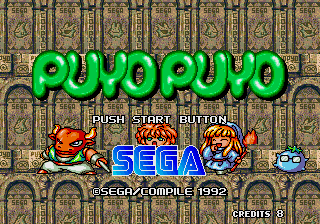
\includegraphics[width=\textwidth]{Puyoarc_e.png} 
	\end{minipage}
	\begin{minipage}{0.48\textwidth}
    {\large Super Off Road}
    \centering
    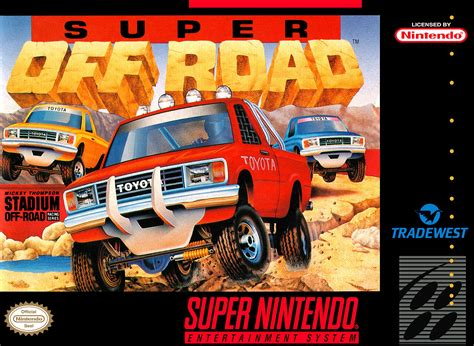
\includegraphics[width=\textwidth]{superOffRoad.jpeg} 
	\end{minipage}
    \vfill
    {\large \@date}
  \end{center}%
  \par
  \vskip 1.5em
  \pagestyle{empty}
  \setcounter{page}{0}
  }
\makeatother

\rmfamily
\renewcommand{\tt}[1]{\texttt{#1}}

\begin{document}

\maketitle
\tableofcontents 
\pagestyle{plain}

\pagebreak

\chapter*{Introduction}

Les jeux analysés dans ce rapport sont Puyo Puyo et Super Off Road. 

Puyo Puyo est un jeu de type puzzle sorti en 1991.

Super Off Road est un jeu de type course sorti en 1989. 

Ce travail de recherche précède un développement des deux jeux, et permet de comprendre en profondeur les différents aspects du programme et comment approcher ce développement. Ainsi, les deux jeux utilisent une boucle itérative pour traiter les informations plusieurs fois par secondes, comme ils sont en temps réel. Dans chaque itération, on traite les informations entrées par le joueur ainsi que l'évolution automatique du jeu avec différents algorithmes spécifiques. 

\chapter{Puyo Puyo}

\section*{Introduction}

Puyo puyo est un jeu vidéo de type puzzle développé par Compile. Il est initialement sorti en 1991 sur console, avant que Sega le commercialise en 1992 sur borne d'arcade. Il est devenu le jeu le plus populaire au Japon avant la sortie de Street Fighter 2. 

Le joueur contrôle deux "Puyo", deux blocs de couleur aléatoires, qu'il peut faire tourner ou déplacer latéralement. Ces blocs sont soumis à la gravité et s'arrêtent lorsqu'ils reposent sur d'autres blocs. Les puyos se collent entre eux s'ils sont de la même couleur, et 4 puyos adjacents ou plus disparaissent, faisant tomber les puyos au-dessus. 

Il existe aussi un mode duel, où un enchaînement effectué par un joueur ralentit l'adversaire. En effet, plus l'enchaînement est long, plus l'adversaire reçoit des blocs gris encombrants qui ne peuvent être détruits qu'en effectuant des nouvelles combinaisons. 


\section{État du jeu}
\subsection{Structure générale et variables}

La structure générale, ne représentant pas un objet du jeu, est : 
\lstinputlisting[language=pdl]{pdl/puyopuyo/Position.txt}

Cette structure permet d'enregistrer la position d'un objet, que ce soit sur la grille en pixels ou dans la matrice avec i et j. 
\\

Les variables générales sont : 
\begin{itemize}
\item constante entier NBCOLORS 
\item constante entier HEIGHT
\item constante entier WIDTH
\item constante entier FALLSPEED 
\item constante entier SIZEPUYO
\item constante entier WIDTHMAT
\item constante entier HEIGHTMAT
\item constante entier WAITINGPOSX
\item constante entier WAITINGPOSY
\item booleen doStartTour
\item booleen gameOver
\item entier penaltyReps1
\item entier penaltyReps2
\\
\end{itemize}

\begin{itemize}
\item[\textbf{constante entier NBCOLORS}] permet de stocker le nombre de couleurs différentes dans le jeu.
\item[\textbf{constante entier HEIGHT}] détermine la hauteur en pixels du plateau de jeu d’un joueur.
\item[\textbf{constante entier WIDTH}] détermine la largeur en pixels du plateau de jeu d’un joueur.
\item[\textbf{constante entier FALLSPEED}] représente la vitesse à laquelle les Puyo tombent.
\item[\textbf{constante entier SIZEPUYO}] représente la taille en pixels d’un côté d’un puyo.
\item[\textbf{constante entier WIDTHMAT}] représente la longueur des lignes de la matrice de blocs.
\item[\textbf{constante entier HEIGHTMAT}] représente la longueur des colonnes de la matrice de blocs.
\item[\textbf{constante entier WAITINGPOSX}]
\item[\textbf{constante entier WAITINGPOSY}] représentent la position de l'affichage des Puyo en attente. 
\item[\textbf{booleen doStartTour}] détermine si un tour va commencer ou non. 
\item[\textbf{booleen gameOver}] est initialisé à faux. Il détermine la fin du jeu.
\item[\textbf{entier penaltyReps1}]
\item[\textbf{entier penaltyReps2}] sont les deux entiers qui prennent chacun en valeur le nombre de malus qu'un joueur recevra au prochain tour. 
\end{itemize}

\subsection{Structure Block}

\lstinputlisting[language=pdl]{pdl/puyopuyo/Block.txt}

Ce type agrégé représente un Puyo, c'est-à-dire un bloc de couleur (variable \tt{color}). Il est stocké dans une matrice \tt{blocks}, qui répertorie la position de chaque bloc. Le booléen \tt{exist} est ici pour savoir si les cases de la matrice sont vides ou non. Afin de connaître les combinaisons de puyos faites sur le jeu, on utilise \tt{groupID} qui attribue un nombre à chaque combinaison. 
\\

\subsection{Structure BlockFall}

\lstinputlisting[language=pdl]{pdl/puyopuyo/BlockFall.txt}

Ce type agrégé représente les 2 Puyo en train de tomber, ceux sur lesquels le joueur peut agir pour changer leur orientation ou leur position sur la grille. Ils possèdent une orientation (\tt{orient}), allant de 0 à 3 (0 pour la gauche, 1 pour le haut, 2 pour la droite et 3 pour le bas). Chaque puyo possède une couleur spécifique (\tt{color1}, \tt{color2} avec comme valeur '\tt{r}','\tt{b}','\tt{g}','\tt{y}' ou '\tt{p}') qui permet de créer des combinaisons de blocs de même couleur. Ils ont également une position (\tt{pos}) sur la grille et une position (\tt{posMat}) dans la matrice de stockage des Puyo. Leur vitesse de chute est déterminée par l'entier \tt{speed}.  
\\

\subsection{Structure Player}

\lstinputlisting[language=pdl]{pdl/puyopuyo/Player.txt}

Le joueur est attaché à une matrice \tt{blocks} dans laquelle sont stockés les Puyo présents sur la grille de jeu. Détruire des combinaisons de Puyo augmentent son \tt{score}. On lui associe aussi un premier BlockFall \tt{bf1} qui est présent sur la grille, et un deuxième BlockFall \tt{bf2} qui est affiché à côté de la grille et qui est le prochain à tomber. 
\\

\subsection{Structure Game}

\lstinputlisting[language=pdl]{pdl/puyopuyo/Game.txt}

Chaque joueur est associé à un jeu (\tt{Game}) de deux joueurs.
\\

\section{Évolution du jeu}

\subsection{Configuration initiale}

\lstinputlisting[language=pdl]{pdl/puyopuyo/startGame.txt}

Le jeu commence avec deux plateaux de jeux vides côte à côte, un pour chaque joueur. La matrice \tt{blocks} de chaque joueur est initialisée avec des blocs vides. Le score des joueurs est à 0, et deux Puyo commencent à tomber sur chaque plateau, en partant du milieu, sur la ligne la plus haute. 

On initialisera aussi un booléen doStartTour à vrai, qui permettra de lancer le premier tour.
\\

\subsection{Règles du jeu}

Le jeu se termine une fois que les nouveaux Puyo ne peuvent plus accéder à la grille d'un joueur, c'est-à-dire quand les deux blocs où ils apparaissent sont déjà occupés par d'autres Puyo qui ne sont pas détruits par combinaisons et lorsque la colonne est remplie d'autres Puyo. Le joueur a alors perdu, et son adversaire gagne. 

\subsection{Actions du joueur}
Le joueur peut effectuer plusieurs actions lors du jeu : il peut déplacer les Puyo en train de tomber sur le côté (on nommera respectivement L et R les touches enfoncées pour déplacer à gauche ou à droite les Puyo), les faire tomber plus vite (touche D) ou changer leur orientation (touches directionnelles). 

Le code 	qui suit est écrit sur la base du joueur 1, on appliquera implicitement ce même code au joueur 2. 

évènement : touche L enfoncée :
\lstinputlisting[language=pdl]{pdl/puyopuyo/leftMotion.txt}

Respectivement, pour la touche R : 
\lstinputlisting[language=pdl]{pdl/puyopuyo/rightMotion.txt}

Ainsi, lorsque le joueur souhaite se déplacer d'un côté, le déplacement sera effectué si le Puyo n'est pas blocké par le bord de la grille de jeu ou par un autre Puyo. 

Évenement : Touche D enfoncée : 
\lstinputlisting[language=pdl]{pdl/puyopuyo/downMotion.txt}

Évenement : Touche D relâchée : 
\lstinputlisting[language=pdl]{pdl/puyopuyo/stopDownMotion.txt}

Lorsque la touche est enfoncée, la vitesse de chute du Puyo est multipliée par 2. Lorsqu'elle est relâchée, elle revient à sa valeur initiale, enregistrée dans \tt{FALLSPEED}. Cette vitesse sera visible dans la partie affichage du jeu, on ne la remarquera donc pas pour le moment.  

Pour changer l'orientation des Puyo en train de tomber, le joueur appuie sur l'une des quatres touches directionnelles. Si le bloc est vide, et qu'il est dans les limites du jeu, alors le changement de direction se fait. 

Événement : Touche directionelle gauche enfoncée : 
\lstinputlisting[language=pdl]{pdl/puyopuyo/leftOrient.txt}

Événement : Touche directionelle haut enfoncée : 
\lstinputlisting[language=pdl]{pdl/puyopuyo/upOrient.txt}

Événement : Touche directionelle droite enfoncée :
\lstinputlisting[language=pdl]{pdl/puyopuyo/rightOrient.txt}

Événement : Touche directionelle bas enfoncée :
\lstinputlisting[language=pdl]{pdl/puyopuyo/downOrient.txt}

C'est ces déplacements qui sont propres au jeu, puisque ce sont eux que le joueur utilisera pour faire ses combinaisons et avancer dans la partie. 
\pagebreak
\subsection{Évolutions automatiques de l’état du jeu}

\subsubsection{initBlockFall}
\lstinputlisting[language=pdl]{pdl/puyopuyo/initBlockFall.txt}

L’action initBlockFall permet d’initialiser un tour en reprenant les valeurs du blockFall suivant, au duo de Puyo, notamment les couleurs et la vitesse. Ensuite, on initialise le duo de Puyo en haut de la matrice. 
\\

\subsubsection{switchColor}
\lstinputlisting[language=pdl]{pdl/puyopuyo/SwitchColor.txt}

Cette fonction retourne un caractère dépendant de l'entier \tt{nb} envoyé en paramètre d'entrée. Ce caractère représente une couleur de Puyo, soit jaune (\tt{yellow}), rouge (\tt{red}), bleu (\tt{blue}), vert(\tt{green}) ou violet (\tt{purple}). La valeur par défaut est \tt{void}, qui est celle affectée aux caractères qu'on ne voit pas. 
\\

\subsubsection{random0toNb}
\lstinputlisting[language=pdl]{pdl/puyopuyo/random0toNb.txt}

Cette fonction retourne un entier aléatoire tiré entre 0 et \tt{nb}. 
\\

\subsubsection{randBlockFall}
\lstinputlisting[language=pdl]{pdl/puyopuyo/randBlockFall.txt}

L’action randBlockFall crée un nouveau BlockFall, avec une orientation égale à 3, c’est-à-dire en bas, deux couleurs aléatoires, initialise sa vitesse, et le positionne à l’emplacement où sera affiché le prochain block qui tombera. On met l'orientation à 3 car il sera affiché vers le bas, mais une fois sur la grille l'orientation sera vers la droite. 
\\

\subsubsection{startTour}
\lstinputlisting[language=pdl]{pdl/puyopuyo/startTour.txt}

La fonction startTour permet d’initialiser un tour. Pour cela, elle fait appel à la fonction initBlockFall pour commencer la descente d'un nouveau duo de Puyos et à la fonction randBlockFall qui crée un nouveau duo de Puyos, indiquant au joueur quel sera le prochain duo. Ensuite, on insère le blockFall dans la matrice, pour que plus tard la fonction \tt{doGravityOnAll}, qui s'appuie sur la matrice, puisse faire tomber le bloc.
\\

\subsubsection{blockTest}
\lstinputlisting[language=pdl]{pdl/puyopuyo/blockTest.txt}

La fonction blockTest retourne un booléen selon l’existence d’un block à l’emplacement indiqué en paramètres d'entrée. Elle retourne vrai s'il n'y a pas de block, faux s'il y en a un.
\\

\subsubsection{doGravityOnAll}
\lstinputlisting[language=pdl]{pdl/puyopuyo/doGravityOnAll.txt}

La fonction doGravityOnAll permet de faire agir une pseudo-gravité sur le jeu. Pour cela, le sous-algorithme teste tour à tour chaque colonne de la matrice représentant le jeu. Pour chacune d’elle, on teste la présence d’un bloc grâce au sous-algorithme blockTest. S’il est retourné vrai, c’est-à-dire si le bloc est vide, tous les éléments de la colonne au-dessus de cette ligne sont « descendus » d’un. Ainsi,  tous les blocs sont maintenant posés au plus bas.
\\

\subsubsection{continueFall}
\lstinputlisting[language=pdl]{pdl/puyopuyo/continueFall.txt} 

La fonction continueFall permet de vérifier si le block en-dessous du duo de Puyo est libre ou non. Il retourne un booléen qui prend la valeur vraie si le block est vide. Pour cela, on prend en compte l'orientation du blockFall.
\\

\subsubsection{blockDown}
\lstinputlisting[language=pdl]{pdl/puyopuyo/blockDown.txt}

L'action blockDown insère le deuxième Puyo du duo de Puyo dans la matrice une fois que le duo termine sa chute. 
\\

\subsubsection{countNbBlocksEqualID}
\lstinputlisting[language=pdl]{pdl/puyopuyo/countNbBlocksEqualID.txt}

La fonction countNbBlocksEqualID permet de retourner la longueur de la chaine auquel appartiennent les blocs possédant un ID égal à l’argument de la fonction.
\\

\subsubsection{AttribuerGroupe}
\lstinputlisting[language=pdl]{pdl/puyopuyo/AttribuerGroupe.txt}

Ici, nous avons un algorithme qui prend en arguments un tableau représentant le jeu du joueur (\tt{Matrice}), la position \tt{posBlock} du block dont on va tester l'appartenance à une chaîne et l'ID de la chaîne (\tt{groupID}). En paramètres de sortie, on aura la matrice avec, pour chaque block, l'ID de la chaîne auquel il appartient ainsi que la longueur de cette chaîne (avec l'ID donné en paramètre). On pourra noter que, s'il n'existe pas de chaîne pour le block à la position \tt{pos}, il ne prendra pas l'ID passé en argument et gardera donc son ID initial. 

Pour le bon fonctionnement de cet algorithme, il faut, avant de le lancer, réinitialiser les ID de tous les blocks à 0 afin que les chaînes soient comptabilisées correctement.
\\

\subsubsection{blockAtStart}
\lstinputlisting[language=pdl]{pdl/puyopuyo/blockAtStart.txt}
Cette fonction vérifie la présence de blocs dans les deux cases où les duos de Puyo sont initialisés. Elle renvoie vrai s'il n'y a aucun block dans cette zone. Elle est utilisée en fin de tour pour vérifier que les blocs d'initialisations sont vides. En effet, s'ils sont pleins, le nouveau duo ne peut pas se générer et la partie se termine.
\\

\subsubsection{checkAllChains}
\lstinputlisting[language=pdl]{pdl/puyopuyo/checkAllChains.txt}

Avec cette fonction, on prend en paramètre le plateau de jeu du joueur qui correspond à une matrice et on vérifie pour chacun des blocks s'il existe et s'il possède un ID différent de 0. Si c'est le cas, on utilise la fonction \tt{AttribuerGroupe} qui permet d'attribuer au block le groupe avec l'ID donné en paramètre de la fonction. Si la chaîne fait plus d'un bloc de long, on lui attribue alors le groupe. Il sera directement changé dans la matrice ainsi que tous les blocks de la chaîne qui la composent. Aussi, s'il y a plus d'un bloc dans la chaîne, on va changer l'ID de la nouvelle chaîne pour avoir deux chaînes bien distinctes. Ainsi, toutes les chaînes de blocks supérieures ou égales à deux auront un identifiant unique dans la matrice.
\\

\subsubsection{resetBlocksForID}
\lstinputlisting[language=pdl]{pdl/puyopuyo/resetBlocksForID.txt}
Cette fonction réinitialise un bloc pour un ID précis donné dans les valeurs d’entrées. Elle vérifie aussi la présence de Puyo blancs à côté, qu'il faut détruire dans ce cas, comme ce sont des blocs malus.
\\

\subsubsection{destroyBlock}
\lstinputlisting[language=pdl]{pdl/puyopuyo/destroyBlock.txt}

La fonction destroyBlock permet de détruire l’ensemble des chaînes de 4 Puyo ou plus, via leur ID. Pour cela, on utilise le sous-algorithme countNbBlocksEqualID en testant tous les ID possibles. Ensuite, la fonction réinitialise l’ensemble des ID des Blocks à 0.
De plus, la fonction compte et retourne le nombre de chaines de Puyo supprimées au cours de la fonction.
\\

\subsubsection{setClearBlocksOnPlayer}
\lstinputlisting[language=pdl]{pdl/puyopuyo/setClearBlocksOnPlayer.txt}

La fonction setClearBlocksOnPlayer permet d’envoyer des malus au joueur sélectionné dans les paramètres d’entrée. Pour chaque malus envoyé (nombre de répétition reps), la fonction tire une colonne aléatoire, d’où le bloc de malus sera créé. Si un bloc est déjà présent en haut de cette colonne, le bloc de malus n'est pas créé. Cela permet de ne pas trop pénaliser le joueur si sa grille est déjà très remplie.  
\\

\subsubsection{boucle Principale}

Encore une fois, l'algorithme s'applique au joueur 1 et s'appliquera implicitement au joueur 2 dans cette boucle principale. 
\lstinputlisting[language=pdl]{pdl/puyopuyo/boucleJeu.txt}

Ainsi, la boucle principale commence par lancer un nouveau tour (au début du jeu, \tt{doStartTour} est initialisé à vrai). Un nouveau duo de Puyo commence à tomber avec la fonction \tt{doGravityOnAll}, et les actions du joueur peuvent modifier sa trajectoire.  
Une fois qu'il se pose sur un Puyo ou au sol (vérifié par la fonction \tt{continueFall}), on regarde s'il a effectué une ou plusieurs combinaisons de 4 Puyo ou plus avec \tt{checkAllChains}. Cela permet ensuite de compter puis détruire ces combinaisons (\tt{destroyBlock}). Selon le nombre de combinaisons effectuées, on incrémente la pénalité de l'autre joueur. On ajoute aussi la pénalité qui a été donnée par l'autre joueur. Enfin, on vérifie que le bloc d'arrivée du duo de Puyo est vide (\tt{blockAtStart}), sans quoi le jeu se termine. Une fonction \tt{gameOver} sera implémentée à la fin de la boucle pour traiter la fin du jeu. 








































\chapter{Super Off Road}

\section*{Introduction}

Super off road est un jeu vidéo de type course développé par Leland Corporation. Il est sorti en 1989 sur borne d'arcade avant d'être adapté sur diverses consoles et ordinateurs. 

Le joueur contrôle un monster truck et doit avancer plus vite que ses 3 concurrents, sur un terrain accidenté qui présente bosses, trous, eau, barrières, montées et descentes qui font accélérer ou ralentir le véhicule. En gagnant, il récupère de l'argent qu'il peut utiliser pour modifier et améliorer son véhicule. 

\section{État du jeu}\subsection{Structures générales et variables}

Les structures générales, ne représentant pas des objets du jeu, sont : 

\subsubsection{Structure Hitbox2P}

\lstinputlisting[language=pdl]{pdl/superOffRoad/Hitbox2P.txt}

La structure \tt{Hitbox2P} permet de stocker deux coordonnées dans le plan, afin de former une hitbox en forme de ligne, notamment utile pour les murs ainsi que pour les flags. 
\subsubsection{Structure Hitbox4P}
\lstinputlisting[language=pdl]{pdl/superOffRoad/Hitbox4P.txt}

La structure \tt{Hitbox4P} est la même que la structure \tt{Hitbox2P}, sauf qu'elle stocke 4 coordonnées et non pas 2, afin de former une hitbox en forme de quadrilatère, notamment en rectangle pour la voiture ou en carré pour les bonus. Les types \tt{corner\_} représentent les sommets de ce quadrilatère.
\\

\subsubsection{Structure Position}

\lstinputlisting[language=pdl]{pdl/superOffRoad/Position.txt}

La structure \tt{Position} permet de stocker les coordonnées d'un point dans le plan, l'entier \tt{x} étant la coordonnée en x et \tt{y} la coordonnée en y.
\\

\subsubsection{Structure Speed}
\lstinputlisting[language=pdl]{pdl/superOffRoad/Speed.txt}

La structure \tt{Speed} stocke la vitesse en x et en y d'une voiture.
\\

Les variables générales sont : 

\begin{itemize}
\item constante entier ACCELERATION
\item constante entier NB\_LAPS
\item constante entier NITRO\_TIME
\item constante entier NITRO\_WIDTH
\item constante entier NITRO\_SPAWN\_TIME
\item constante entier CAR\_WIDTH
\item constante entier CAR\_HEIGHT
\item Car playerCar
\item Bonus [] nitroList
\item entier malusBonusSpeed <- 1
\\
\end{itemize}

\begin{itemize}
  \item [\textbf{constante entier ACCELERATION}]permet de stocker l'accélération de référence de la voiture.
  \item [\textbf{constante entier NB\_LAPS}]permet de stocker le nombre de tours demandés pour finir la course et gagner la partie.
  \item[\textbf{constante entier NITRO\_TIME}]permet de stocker le temps durant lequel le boost de vitesse donné par la nitro est actif.
  \item[\textbf{constant entier NITRO\_WIDTH}]stocke la longueur d'un côté de la hitbox du bonus de nitro.
  \item[\textbf{constante entier NITRO\_SPAWN\_TIME}]stocke le temps entre chaque génération d'un bonus de nitro sur la carte.
  \item[\textbf{constante entier CAR\_WIDTH}]
  \item[\textbf{constant entier CAR\_HEIGHT}]permettent de stocker respectivement la longueur et la largeur de la hitbox de la voiture.
  \item[\textbf{Car playerCar}]Cette variable de type \tt{Car} va stocker toutes les informations relatives à la voiture du joueur (sa position, sa vitesse, sa direction\ldots)
  \item[\textbf{Bonus [] nitroList}]Ce tableau de variable de type \tt{Bonus} permet de stocker les information relative a l'emplacement des bonus de nitro présents sur la map.
  \item[\textbf{entier malusBonusSpeed <- 1}]Cet entier stocke un multiplicateur de l'accélération, permettant d'influencer sur la vitesse de la voiture lorsque celle-ci rencontre un mur ou de la boue.
\end{itemize}

\subsection{Structure Flag}

\lstinputlisting[language=pdl]{pdl/superOffRoad/Flag.txt}

Les flags sont des lignes invisibles que le joueur traversera durant la course. Ceux-ci permettent de confirmer que le joueur effectue la course dans le bon sens, pour éviter un bug qui consisterait à se retourner et passer la ligne d'arrivée trois fois d'affilées, sans faire la course complète. 

Le type structuré \tt{hitbox} contient les deux coordonnées qui délimitent les extrémités de la hitbox et de la position du Flag. Le type \tt{nb} contient l'ordre du flag sur le trajet du joueur (0 pour la ligne de départ et d'arrivée, 1 pour le premier flag traversé par le joueur, etc\ldots).
\\
\pagebreak
\subsection{Structure Wall}

\lstinputlisting[language=pdl]{pdl/superOffRoad/Wall.txt}
Les \tt{Wall} sont les éléments du décors qui délimitent les bordures du circuit de course. Dans ce type structuré, on trouve le type structuré \tt{hitbox2P} qui permet de stocker les deux points qui forment les extrémités de la hitbox du mur ainsi que sa position. Nous trouvons aussi l'entier \tt{directionStop} qui stocke la direction dans laquel la voiture du joueur doit arriver pour être stoppée nette et non pas redirigée (cette direction est colinéaire à la normale de la ligne qui forme la hitbox du mur).
\\

\subsection{Structure Car}

\lstinputlisting[language=pdl]{pdl/superOffRoad/Car.txt}

Car est un type structuré possédant une position \tt{pos} dans l'espace de jeu, une vitesse \tt{speed} du tour précédent permettant le déplacement de la voiture ainsi que le calcul de la vitesse au tour suivant. On a une direction \tt{direction} qui est un entier entre 0 et 15 compris. Il permet de diriger la voiture selon 16 directions définies. L'entier \tt{flag} permet de garder en mémoire la valeur du dernier drapeau traversé lorsqu'il est supérieur au précédent. L'entier \tt{laps} quant à lui garde en mémoire le nombre de tours du véhicule en fonction du nombre de \tt{flag}. On a ensuite la \tt{hitbox} de la voiture permettant de gérer ses collisions avec d'autres objets du jeu. Enfin, nous avons un entier \tt{nbNitro} qui s'occupe de gérer les Nitros utilisables par le joueur.
\\

\subsection{Structure Bonus}

\lstinputlisting[language=pdl]{pdl/superOffRoad/Bonus.txt}
La structure \tt{Bonus} permet de stocker les informations de position d'un bonus, avec le type \tt{pos} ainsi que sa hitbox avec le type \tt{hitbox}.
\\

\subsection{Structure Mud}

\lstinputlisting[language=pdl]{pdl/superOffRoad/Mud.txt}
La structure \tt{Mud} permet de stocker la position (\tt{pos}) d'un obstacle de boue et sa \tt{hitbox}.
\\

\subsection{Structure Ground}
\lstinputlisting[language=pdl]{pdl/superOffRoad/Ground.txt}

La structure \tt{Ground} est une structure de stockage de données qui contient les informations sur le niveau. On y trouve les \tt{walls} qui permettent de gérer les collision avec les murs de la piste, \tt{spawnPosNitro} qui sont les lieux où peuvent apparaître les boîtes de Nitro, \tt{muds} sont les zones où sont disposées les mares de boues qui ralentissent les voitures ainsi que les \tt{flags} qui sont là pour compter les tours et éviter de tricher en faisant les tours par l'arrière.
\\

\section{Évolution du jeu}

\subsection{Configuration initiale}

\lstinputlisting[language=pdl]{pdl/superOffRoad/InitialisationProgram.txt}
Dans la phase d'initialisation du jeu, on effectue la déclaration de plusieurs variables très utiles :

\begin{itemize}
\item
Le réel \tt{timer} permet de ne faire apparaître un bonus qu'à certains intervalles de temps,
\item
La variable \tt{level} de type \tt{ground} stocke les listes de tous les objets importants du jeu,
\item
La liste de tous les murs (\tt{level.walls}) qui nécessite d'être précisée à la main pour que les hitboxs et positions des murs correspondent avec le background,
\item
La liste de tous les flags (\tt{level.flags}), là encore cette liste sera précisée plus tard pour correspondre avec le circuit, 
 \item
La liste \tt{level.muds}, précisée plus tard
 \item
La liste \tt{level.spawnPosNItro} qui contient les emplacements possibles d'apparition des bonus de nitro,
\item
La variable \tt{playerCar} de type \tt{Car} qui stocke les informations contenant la voiture du joueur. Sa position en x et en y sera précisée pour correspondre avec la ligne de départ du circuit, 
\item
La vitesse (\tt{playerCar.Speed}) de la voiture est initialisée à 0, 
\item
Similairement pour le nombre de tours effectués (\tt{playerCar.laps}),
\item
Le nombre de flags franchis (\tt{playerCar.flag}), encore une fois initialisé à 0
\item
Le nombre de nitro disponible au début de la course est fixé à 3 (\tt{playerCar.nbNitro}),
\item
Les booléens \tt{haut}, \tt{bas}, \tt{gauche}, \tt{droite}, et \tt{nitro} sont des variables qui vont stocker les actions effectuées par le joueur lorsqu'il appuie sur les touches, permettant de modifier l'état du jeu. Par défaut, ces variables sont initialisées à faux.
\end{itemize}

Voila pour l'initialisation du jeu.

\subsection{Règles du jeu}

Super Off Road est un jeu de course de voiture dont le but est d'être le premier à compléter 3 tours d'un circuit en terre. Ce circuit comporte des obstacles tels que des bosses, des montées et descentes, des flaques de boue et autres, impactant la vitesse du joueur. Le circuit est délimité par des palissades infranchissables. Pour être le premier, le joueur dispose avant la course d'une certaine quantité d'argent qu'il peut utiliser pour s'acheter des améliorations comme un moteur plus puissant, des roues plus adhérentes ou de la nitro utilisable pendant la course pour s'octroyer un boost de vitesse temporaire.
\\

\lstinputlisting[language=pdl]{pdl/superOffRoad/ReglesDuJeuMurs.txt}

Le premier test réalisé dans la boucle sera celui de la rencontre entre la voiture et le mur. Ceci sera testé avec la fonction \tt{isCollision}. S'il y a bel et bien collision, on utilise la fonction \tt{redirectIfPunchWall}, lui donnant en argument cette voiture et le mur que l'on a heurté. Cela permet de changer la direction de la voiture. On calcule ensuite sa vitesse avec le nouvel angle, et on finit par apppliquer un malus de vitesse avec \tt{malusBonusSpeed}.

Pour simplifier, cette boucle vérifie la collision avec un mur et, si c'est le cas, on réajuste la direction et la vitesse de la voiture.
\\

\lstinputlisting[language=pdl]{pdl/superOffRoad/ReglesDuJeuMuds.txt}

On teste si notre voiture est dans une mare de boue en vérifiant la collision entre la hitbox de la voiture et chacune des hitboxs des mares. On utilise la même fonction que précédemment \tt{isCollision} pour vérifier cela. Ainsi, être dans la boue signifie une réduction de vitesse de 0.20\%
\\

\lstinputlisting[language=pdl]{pdl/superOffRoad/ReglesDuJeuRecupererNitro.txt}

On continue les tests, cette fois-ci en regardant les boîtes de Nitro. Si la voiture les a touchées, ce qu l'on vérifie encore une fois grâce à \tt{isCollision}, on ajoute à notre voiture une Nitro supplémentaire, et la boîte qui vient d'être prise est supprimée de l'affichage.
\\

\lstinputlisting[language=pdl]{pdl/superOffRoad/ReglesDuJeuSetSpeedAuto.txt}

On appelle ensuite la fonction \tt{calculateSpeed} qui va s'occuper de calculer la vitesse en fonction des différents obstacles qui ont déjà été pris en compte. On prendra aussi en paramètres les événements de l’utilisateur pour modifier la vitesse de la voiture.
\\

\lstinputlisting[language=pdl]{pdl/superOffRoad/ReglesDuJeuNitroSpawn.txt}

Si le temps est écoulé entre deux apparitions de Nitro (définie par NITRO\_SPAWN\_TIME) on vérifie si la liste de d'apparition \tt{nitroList} possède des points d'apparition libres (qui ont des coordonnées de (0, 0). S'il reste un espace libre, alors on appelle la fonction \tt{generateNitro} qui permet de récupérer l’objet \tt{Bonus} qui sera positionné dans un emplacement libre de la carte.

\lstinputlisting[language=pdl]{pdl/superOffRoad/ReglesDuJeuFlag.txt}

On utilise des drapeaux disséminés dans la carte pour vérifier que les  voitures effectuent les tours dans le bon sens, afin d'éviter une exploitation de bugs. On assigne à chaque drapeau un nombre, dans l'ordre croissant, et on oblige le joueur à passer par chaque drapeau pour valider un tour. Ainsi, lorsqu'il passe un drapeau, on peut vérifier s'il effectue correctement son tour. On utilise la fonction \tt{countTour} pour gérer le nombre de tours de la voiture.

\lstinputlisting[language=pdl]{pdl/superOffRoad/ReglesDuJeuMoveCar.txt}

On appelle simplement la fonction \tt{moveCar} qui va déplacer la voiture en fonction de la vitesse enregistrée dans le type structuré.


\subsection{Actions du joueur}


\lstinputlisting[language=pdl]{pdl/superOffRoad/ActionDuJoueur.txt}

Les actions que le joueur peut effectuer sont les suivantes : il peut apuyer sur la touche z, ce qui mettra le booléen \tt{haut} à vrai jusqu'à ce qu'il la relâche, cela a pour effet de faire accélérer la voiture; il peut appuyer sur la touche q, ce qui mettra le booléen \tt{gauche} à vrai (toujours jusqu'à ce qu'il la relâche). Ce booléen aura pour effet d'incrémenter la variable \tt{playerCar.direction} de -1, résultant en une rotation de la voiture vers la gauche.
Il peut appuyer sur la touche s, pour mettre la variable \tt{bas} à vrai. Cela fera freiner la voiture. 
Il peut appuyer sur la touche d, ce qui mettra la variable \tt{droite} à vrai, ce qui incrémentera la direction de 1 et fera tourner la voiture vers la droite.
Et enfin, il peut appuyer sur la barre espace pour passer le booléen \tt{nitro} à vrai et donc consommera une charge de nitro pour accorder un boost de vitesse temporaire.
\\

\subsection{Algorithmes}

\subsubsection{redirectIfPunchWall}
\lstinputlisting[language=pdl]{pdl/superOffRoad/redirectIfPunchWall.txt}

Cet algorithme prend en paramètres la voiture qui a touché le mur (\tt{car}) et le mur touché (\tt{wall}). Elle renvoie un entier entre 0 et 15 qui correspond à la nouvelle direction de la voiture. On peut calculer la redirection de la voiture grâce a la direction que bloque le mur. 

\subsubsection{calculateNorme}
\lstinputlisting[language=pdl]{pdl/superOffRoad/calculateNorme.txt}

Cette fonction calcule la norme d'un vecteur à partir de sa longueur en \tt{x} et en \tt{y} et renvoie un réel correspondant à cette norme.
\\
\subsubsection{calculateSpeed}
\lstinputlisting[language=pdl]{pdl/superOffRoad/calculateSpeed.txt}

Cette fonction prend en paramètres la voiture dont on veut calculer la vitesse (\tt{car}), l'accéleration de cette voiture (\tt{acceleration}, l'accélération standard (\tt{avgAcceleration}) et le temps depuis la dernière itération (\tt{dt}). Nous avons décidés de rajouter \tt{isAccelerate}, \tt{isBreack} et \tt{isNitro} pour permettre une meilleure interaction de la vitesse avec le joueur. On calcule d'abord l'angle de la voiture grâce à la direction de celle-ci puis sa vitesse normalisée afin d'avoir une seule composante.
On vérifie la touche accélération est enfoncée, si ce n'est pas le cas on va faire ralentir la voiture.
Si on utilise de la Nitro la vitesse passe immédiatement à 1,20 fois celle maximum et on la renvoie.
Si on décide de break alors on divise par 3 notre précédente vitesse, qu'on met à 0 si elle est à moins de 20\%.
Si aucune de ces condition n'a été validée alors on accélère normalement (pleine vitesse en 5~-~6s). Sinon on ralenti fortement (0 en 3~-~4s). La fonction retourne la nouvelle vitesse.
\\

\subsubsection{moveCar}

\lstinputlisting[language=pdl]{pdl/superOffRoad/moveCar.txt}

Cette fonction simple modifie la position de la voiture en fonction du temps écoulé depuis la dernière itération (\tt{dt}) ainsi qu'en utilisant sa vitesse.
\\

\subsubsection{getProject}

\lstinputlisting[language=pdl]{pdl/superOffRoad/getProject.txt}

Cette fonction prend en entrées un vecteur unitaire et un ensemble de point. Elle calcule la projection de chacun des points de la liste sur la droite portée par le vecteur unitaire grâce à un produit scalaire. Cette fonction retourne ainsi une liste de réels qui correspondent chacun à l'emplacement de la projection des points sur la droite. 
\\

\subsubsection{getAxisList}

\lstinputlisting[language=pdl]{pdl/superOffRoad/getAxisList.txt}

Cette fonction prend en entrées un tableau de points dans le plan, formant un polygone convexe. 
Pour chaque arête de ce polygone, la fonction calcule le vecteur unitaire normal à la droite formée par l'arête. 
Cet algorithme retourne une liste de vecteurs unitaires normaux à une arête du polygone.
\\

\subsubsection{isCollisionAxis}

\lstinputlisting[language=pdl]{pdl/superOffRoad/isColisionAxis.txt}

Cette fonction va prendre en paramètres d'entrée deux liste de points correspondant aux sommet des deux polygones convexes que l'on veut tester ainsi que le vecteur unitaire selon lequel on veux tester la collision. Concrètement, la fonction va projeter tout les sommets du premier polygone sur la droite, cela à l'aide de la fonction \tt{getProject}, puis répète ce traitement pour le second polygone. Ensuite, on teste la potentielle superposition des deux listes de réels, c'est-à-dire si le maximum d'une liste est supérieur au minimum de l'autre liste, et inversement. 
Si cette liste se superpose, alors il y a collision sur cette axe, sinon, il n'y pas collision.
Cette fonction retourne donc un booléen, vrai si il y a collision, faux sinon.
\\

\subsubsection{isCollision}

\lstinputlisting[language=pdl]{pdl/superOffRoad/isColision.txt}

Cette fonction va juste tester si deux polygones sont en collision à l'aide du théorème des axes séparateurs. \footnote{\url{https://www.sevenson.com.au/programming/sat/}}
%lien vers le site
Il va donc prendre en entrées deux listes de points représentant les sommets de deux polygones pour calculer la liste de toutes les normales d'un polynome avec la fonction \tt{getAxis}. Puis, pour chaque normale, on projete les sommet des polygones et on vérifie s'il y a collision avec la fonction \tt{isCollisionAxis}. S'il y a collision entre les deux polynomes pour toutes les normales, alors il y collision entre les deux polynomes, sinon il n'y a pas collision entre les deux polynomes.
Cette fonction retourne donc un booléen, vrai si les deux polynomes sont en collision, faux sinon.
\\

\subsubsection{hitbox\_toList}

\lstinputlisting[language=pdl]{pdl/superOffRoad/ToList.txt}

Ces deux fonctions permettent de transformer les \tt{Hitbox4P} et les \tt{Hitbox2P} en des listes de points. Ces listes de points sont utilisées dans la fonction \tt{isCollision} pour détecter si une collision a lieu.
\\

\subsubsection{getHitboxCar}

\lstinputlisting[language=pdl]{pdl/superOffRoad/calculDeLaHitbox.txt}

Cette fonction calcule les positions des sommets de la voiture en fonction de son orientation, de sa longueur et de sa largeur, tout cela à l'aide de trigonométrie élémentaire.
\\

\subsubsection{countTour}
\lstinputlisting[language=pdl]{pdl/superOffRoad/countTour.txt}

Cette fonction prend comme argument une voiture \tt{car}, le drapeau \tt{flag} qu'elle vient de franchir et le nombre de drapeaux que possède la carte. On vérifie d'abord si le drapeau est le premier drapeau d'indice 0. Dans ce cas, on vérifie que l'on a fait le tour de tous les drapeau donc que le \tt{flag} de notre voiture a parcouru tous les autres drapeau (flag == nbFlags -1). Dans ce cas on compte un tour et on renvoie ce nombre. Sinon, on vérifie que le drapeau est bien celui qui devait être passé par la voiture (donc que son indice est plus élevé de 1). Si ce n'est pas le cas, on ne change pas l'indice de son drapeau.
\\

\subsubsection{vectorDotProduct}

\lstinputlisting[language=pdl]{pdl/superOffRoad/vectorDotProduct.txt}

Cette fonction retourne le produit scalaire de deux vecteurs.
\\

\subsubsection{spawnNitro}

\lstinputlisting[language=pdl]{pdl/superOffRoad/generateNitro.txt}

Cette fonction va prendre en arguments la liste des endroits où peut apparaître de la nitro, ainsi que la liste des endroits où des bonus de nitro sont déjà présents. Elle peut ainsi générer un nouveau bonus de nitro avec une position différente de ceux déjà présents dans la liste.

\chapter*{Conclusion}
\addcontentsline{toc}{chapter}{Conclusion}

Pour conclure, nous pouvons énoncer les différences et points communs de ces deux jeux. Au cours de ce rapport nous avons pu voir que le fonctionnement de ces jeux est fondamentalement différent. En effet, tandis que Puyo-puyo est un jeu de type puzzle, Super off road est de type course. Par conséquent, de nombreuses lois sont différentes, notamment l’utilisation d’une “gravité” dans le premier, totalement inexistante dans le second. Aussi, contrairement à Super off road qui peut être joué à 1, 2, 3 ou 4 joueurs, Puyo-Puyo ne présente qu'un mode 2 joueurs. De plus, on constate que le but de ces jeux ne sont pas les mêmes. Dans Puyo-puyo, pour l’emporter, il faut battre le joueur adverse, en lui envoyant des malus, tandis que pour Super Off Road, le joueur doit gagner toutes les courses afin de terminer le jeu. De ce fait, Puyo-puyo ne possède pas de “fin” en soi. 

On observe malgré tout dans ces deux jeux certains points communs, par exemple, l’existence d’un moyen d’accélérer l’élément contrôlé par le joueur, ou encore de le déplacer avec les flèches sur la map en 2D. 
L’existence d’un système de malus est aussi présent dans les deux jeux. Cependant, tandis que les malus sont donnés par le second joueur dans Puyo-puyo, les obstacles sont générés par la carte elle-même dans Super Off Road. 


\begin{abstract}

Dans ce rapport, vous trouverez l'analyse structurelle des deux jeux suivants : Puyo Puyo et Super Off Road. Ce rapport sera divisé en deux parties, chacune traitant de l'un des deux jeu. Chacune de ces parties sera elle même divisée en deux sous-parties, l'une traitant de l'état du jeu (structures et variables qui le composent), et l'autre traitant de l'évolution du jeu (règles du jeu, actions du joueur, initialisation). Ce rapport a été fait dans le cadre du cours de Projet Ingénieurie du CMI informatique.
\\

In this report, you will find the structural analysis of the following two games : Puyo Puyo and Super Off Road. This report will be divided into two chapters, each one treating one of the two games. Each of those parts will also be divided in two subparts, one dealing with the state of the game (structures and variables composing it), and the second one dealing with the evolution of the game (rules, actions from the player, initialization). This report was redacted during the course of a Computer Science Engineering project. 
\end{abstract}

\end{document}
